\newcommand{\PayloadEligible}{27}
\newcommand{\PayloadControls}{81}
\newcommand{\PayloadPowerMin}{94.54}
\newcommand{\PayloadPowerMax}{95.39}
\newcommand{\PayloadLodMin}{0.287}
\newcommand{\PayloadLodMax}{400.598}

\section{Payload information, sensitivity and limits}
\noindent\textbf{Critical calibration assumption.} Favorable results assume zero residual calibration error after correction; this accuracy has not been established experimentally. Receiver noise and finite reference uncertainty remain present. At 45 degrees in the standard atmosphere, with 10 s reference plus 10 s sample, predicted acetonitrile recall at 1 \ugm\ is 93.84\%, 92.55\% and 25.17\% for differential residual standard deviations of 0, 0.0001 and 0.001 dB, respectively. These are correlated random error scenarios, not measured calibration statistics or worst case drift guarantees. A 0.001 dB power deviation is approximately 0.023\%. Persistent systematic drift cannot be removed by longer averaging alone.
\subsection{Unknown data, noise and finite reference}
For $y=\sqrt{S}x+w$, equiprobable unit QPSK $x$ and $w\sim\mathcal{CN}(0,V)$, the parameters are $u=\log S$ and $v=\log V$. Each real coordinate has a symmetric BPSK mixture density, connecting the analysis to non data aided estimation~\cite{nda}. With $a=\sqrt{S/2}$ and $t=2ar/V$, its scores are
\begin{align}
g_u&=-a^2/V+(ar/V)\tanh t,\\
g_v&=-1/2+(r^2+a^2)/V-t\tanh t.
\end{align}
The full QPSK information is $J=2\mathbb E[gg^\top]$. An unknown constant phase is orthogonal to these parameters by symmetry; arbitrary untracked phase instead requires the magnitude observation. For $q=|y|^2$, the Rice likelihood~\cite{rice} is
\begin{equation}
p(q)=V^{-1}e^{-(q+S)/V}I_0(2\sqrt{qS}/V).
\end{equation}
Both likelihoods profile unknown receiver noise through $j=J_{uu}-J_{uv}^2/J_{vv}$. With $k=10/\ln 10$, the local attenuation variance bound is $k^2/(Nj)$. Independent finite sample and reference windows give
\begin{equation}
\operatorname{var}(\widehat A)\geq k^2\left[(N_sj_s)^{-1}+(N_rj_r)^{-1}\right].
\end{equation}
This follows by eliminating their shared unknown baseline power and separate noise powers. A direct joint Fisher inverse verifies it. Equal SNRs favor equal time allocation at fixed total budget.

Per tone information is propagated through the joint concentration and spectral nuisance design using whitened projection and normalized SVD. The information order is known symbols, full QPSK, magnitude, then M2M4, in increasing variance. Numerical quadrature refinement and independent density derivatives verify the scores. These are local regular estimation bounds, not universal detection bounds or biased-estimator MSE guarantees.

\begin{table}[t]\centering\footnotesize
\caption{Charged 10 s reference plus 10 s sample, standard atmosphere at 45 degrees, zero residual. Efficiency is joint full-QPSK CRLB variance divided by M2M4 variance.}
\begin{tabular}{lrrr}\toprule
Gas & Limit (\ugm) & Limit (ppm) & Efficiency\\\midrule
Formaldehyde & 4.456 & 0.003509 & 95.9\%\\
Methanol & 10.307 & 0.007606 & 97.6\%\\
Acetonitrile & 1.023 & 0.000589 & 96.5\%\\
\bottomrule\end{tabular}

\label{tab:payloadbounds}
\end{table}
M2M4 already retains about 96--98\% of the full constellation information in this reference. Estimator replacement therefore offers limited improvement under these assumptions. The limits in Table~\ref{tab:payloadbounds} account for concentration dependent sample noise before validation. They are surface equivalent enhancements under the assumed vertical profile. Ppm conversion uses local surface temperature, pressure and natural mixture molar masses.

\subsection{Elevation, weather and changing geometry}
The physical sweep recomputes refracted paths, Voigt spectra, background absorption, sky emission, receiver SNR and communication water filling at six elevations from 5 to 90 degrees, for the standard atmosphere and four selected IGRA soundings. All 21 recovered HITRAN isotope files match their previous raw hashes. Durations of 2, 20 and 100 s include equal reference/sample windows. Additional scenarios double receiver noise or introduce 0.0001 and 0.001 dB correlated differential calibration residuals. Frequencies and decision thresholds are fixed.

At nominal receiver noise, \PayloadEligible{} of 30 cases retain at least 20 tones above the fixed 5 dB gate. Failed operating points remain explicit. Each eligible 20 s case has 10,000 null responses and 10,000 responses for each VOC at its predicted 95\%-power limit. Across \PayloadControls{} controls, observed power is \PayloadPowerMin--\PayloadPowerMax\%, using nonlinear moment inversion with the previously tested joint moment approximation. Exact binomial intervals and all response arrays are retained. There is no threshold tuning on these trials.

Acetonitrile limits across eligible matched weather cases span \PayloadLodMin--\PayloadLodMax\ \ugm. At standard atmosphere and 20 s, its predicted recall at 1 \ugm\ changes from 48.17\% at 30 degrees to 93.84\% at 45 degrees and 99.92\% at zenith. The weather supplied to retrieval is correct in this sweep; previously observed weather mismatch biases remain unresolved.

\begin{figure*}[t]\centering
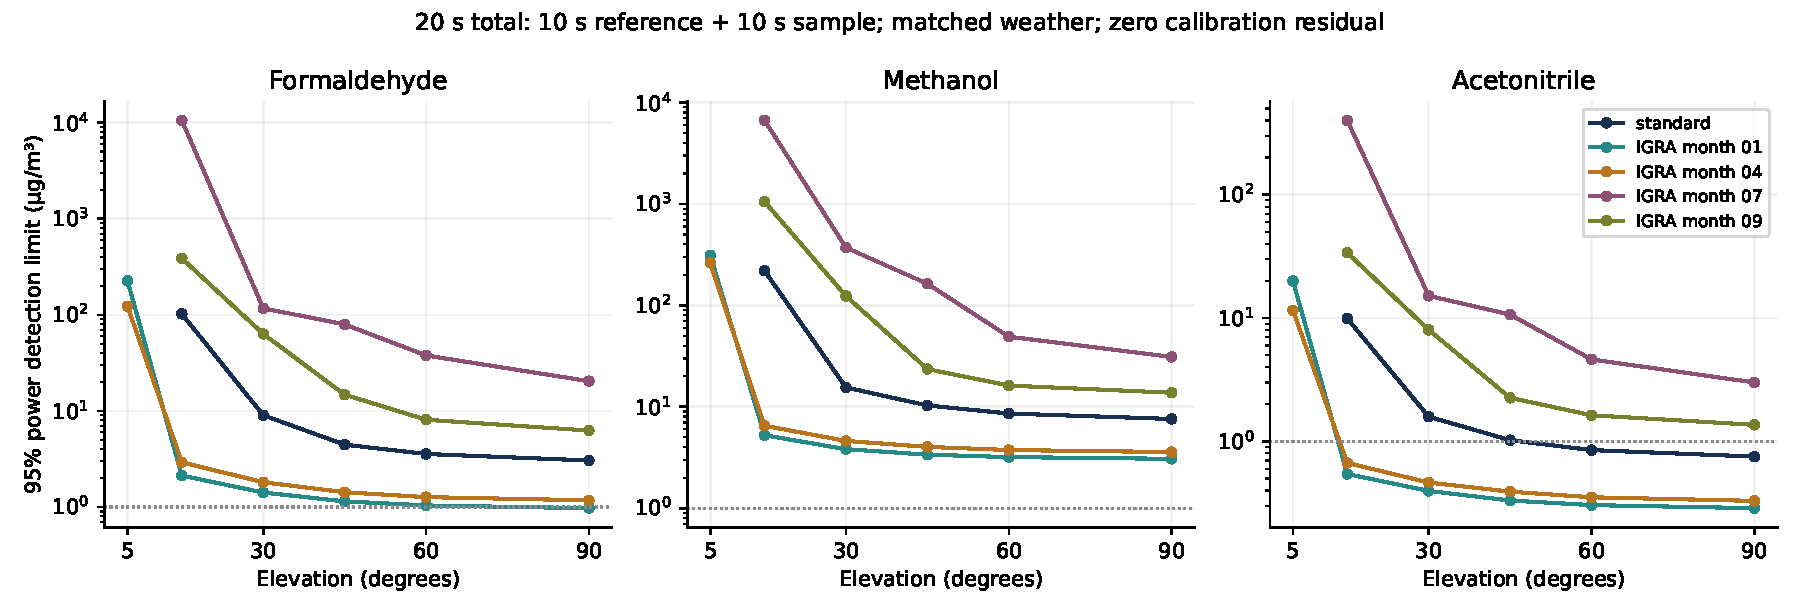
\includegraphics[width=0.97\textwidth]{../results/payload_bounds/payload_operating_region.pdf}
\caption{Matched weather operating region with a charged finite reference. Gaps fail the fixed SNR and usable tone gate. The dotted line is 1 \ugm. These are modeled enhancement limits, with zero differential calibration residual and assumed pollutant vertical profiles.}
\label{fig:payloadregion}
\end{figure*}

Time dependent information is also integrated along an ideal overhead circular 550 km orbit, with shared concentrations and independent block nuisance coefficients. Matched reference and sample passes both consume transmission resources. At 20 s total, acetonitrile local limits are 1.027 \ugm\ around 45 degrees and 0.753 \ugm\ around zenith. Doubling the time quadrature changes standard deviations by less than 0.05\%. This assumes accurate instantaneous gain normalization and matched atmosphere; orbital waiting time is excluded. It does not implement synchronization, Doppler tracking or a moving waveform receiver.

\subsection{Standards and unresolved requirements}
The WHO 2021 ambient guidelines do not provide methanol or acetonitrile thresholds~\cite{who2021}. Formaldehyde's 100 \ugm, 30 minute indoor guideline~\cite{who2010} is not a satellite slant-column compliance threshold. PM2.5 and PM10 daily guideline values of 15 and 45 \ugm\ also differ in averaging time and measurement domain, while modeled PM information remains inadequate. Improved detection limits therefore do not establish environmental compliance.

The added evidence addresses the payload extensions of proposal Tasks 4.1--4.3 under declared assumptions. The principal next requirements are an implementable multiband resource configuration and a calibrated moving receiver, Tasks 2.1--2.2. Joint useful PM retrieval and independent physical concentration validation remain open.
